\documentclass[
    NAME={Dr. Helga Ingimundardóttir},
    EMAIL={helgaingim@hi.is},
    FACULTY={Industrial Engineering},
    TITLE={Mixed Integer Programming},
    SUBTITLE={Techniques and Applications},
    SEMINAR={VÉL113F},
    DATE={Design and Optimization},
    WIDE=true
]{../HI-latex/hi-beamer}

\let\oldframe\frame
\renewcommand\frame[1][allowframebreaks]{\oldframe[#1]}
\usepackage{IEEEtrantools}
\begin{document}
    \begin{frame}{Introduction}
        \begin{block}{Integer Programming (IP)}
            Exploring the complexities of optimization when decision variables are limited to discrete values. Integer and
            discrete programming offer solutions when continuity is not feasible.

            \small
            \begin{itemize}
                \item IP deals with optimization problems where some or all of the variables are restricted to be integers.
                \item Common in situations where solutions involving fractions or decimals are not feasible, such as
                in task scheduling or determining quantities of products to manufacture.
                \item Generally harder to solve than their LP counterparts due to the discrete nature of solutions.
            \end{itemize}
        \end{block}

        An IP in which only \emph{some} of the variables are required to be integers is called a \emph{mixed integer
        programming problem}.


    \end{frame}

    \begin{frame}{Assumptions of Linear Optimization}
        To apply traditional linear optimization, the following assumptions are made:
        \begin{description}
            \item[Proportionality] The contribution of product $j$ to the objective function is proportional to
            the value of $x_j$. The same applies to the left-hand side in constraints.
            \item[Additivity] The objective function and the left-hand side of constraints are the sum of
            contributions from individual products. E.g., $ z = 3x_1 + 5x_2 + x_1x_2 $.
            \item[Divisibility] Decision variables can take any real value within the solution area.
            \item[Certainty] We assume that the values of the parameters $ a_{ij}, b_i $ and $ c_j $ are fully
            known.
        \end{description}
    \end{frame}

    \begin{frame}{Linear Programming Example}
        \begin{columns}
            \begin{column}{0.5\textwidth}
                \begin{example}[Wyndor-Glass Company]
                {\small
                Wyndor, a glass product manufacturer, plans to start producing two new types of products which can be made in three different factories.
                    \begin{itemize}
                        \item Product 1: Produced in factories 1 and 3
                        \item Product 2: Produced in factories 2 and 3
                    \end{itemize}

                    Everything that is produced can be sold.}
                {\centering \footnotesize
                    \begin{tabular}{|cccc|}
                        \hline
                        Factory & \multicolumn{2}{c}{Production Time (hrs)} & Available Time \\
                        & Product 1 & Product 2 &    \\
                        \hline
                        1      & 1         & 0         & 4  \\
                        2      & 0         & 2         & 12 \\
                        3      & 3         & 2         & 18 \\
                        \hline
                        Profit & \$3000    & \$5000    &    \\
                        \hline
                    \end{tabular}
                }
                \end{example}

            \end{column}
            \begin{column}{0.5\textwidth}
                \begin{figure}

                    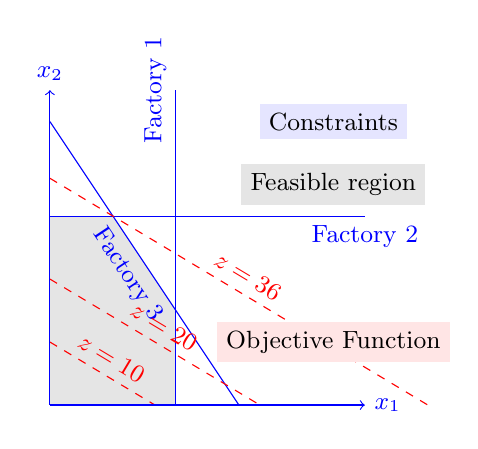
\begin{tikzpicture}[scale=0.4,every node/.style={font=\small}]
                        % Filling the feasible region
                        \fill[gray!20] (0,0) -- (0,6) -- (2,6) -- (4,3) -- (4,0) -- cycle;

                        % Constraints
                        % Factory 1: x1 <= 4
                        \draw[blue] (4,0) -- (4,10) node[at end, above, sloped] {Factory 1};
                        % Factory 2: x2 <= 6
                        \draw[blue] (0,12/2) -- (10,12/2) node[at end, below, sloped] {Factory 2};
                        % Factory 3: 3x1 + 2x2 <= 18
                        \draw[blue] (0,9) -- (6,0) node[midway, below, sloped] {Factory 3};

                        % Objective function lines (derived)
                        % z = 3x1+5x2, then x2=z/5+3/5x1
                        % Here, I'll simplify things by plotting the lines for z=10, z=20, z=36
                        \foreach \z in {10,20,36} {
                            \draw[red,dashed] (0,{\z/5}) -- ({\z/3},0) node[midway,above,sloped] {\small \(z = \z\)};
                        }

                        % Legends
                        \node at (9,9) [rectangle,fill=blue!10] {Constraints};
                        \node at (9,2) [rectangle,fill=red!10] {Objective Function};
                        \node at (9,7) [rectangle,fill=gray!20] {Feasible region};

                        % Axis
                        \draw[blue,->] (0,0) -- (10,0) node[right] {$x_1$};
                        \draw[blue,->] (0,0) -- (0,10) node[above] {$x_2$};

                    \end{tikzpicture}
                    \caption{Graphical solution.}
                \end{figure}
            \end{column}
        \end{columns}


        \begin{columns}
            \begin{column}{0.5\textwidth}
                \begin{example}[Wyndor-Glass Company]
                {\small
                Let's explore a simplified scenario for the Wyndor-Glass Company. Suppose we only consider the
                constraint $x_1\leq 4$ and disregard all other constraints. With this sole constraint, what is the
                maximum profit achievable from the production of the products}
                \end{example}

            \end{column}
            \begin{column}{0.5\textwidth}
                \begin{figure}

                    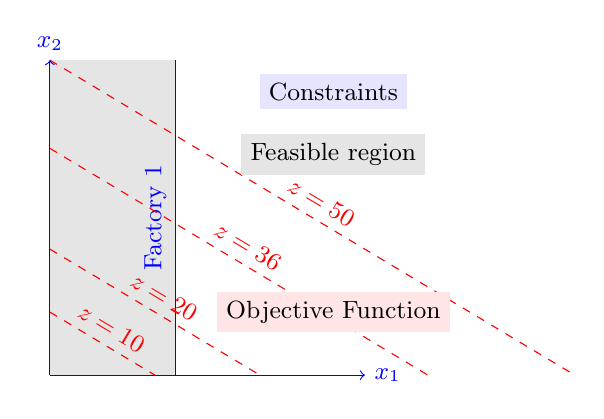
\begin{tikzpicture}[scale=0.4,every node/.style={font=\small}]
                        % Filling the feasible region
                        \fill[gray!20] (0,0) -- (0,10) -- (4,10) -- (4,0) -- cycle;

                        % Constraints
                        % Factory 1: x1 <= 4
                        \draw[blue] (4,0) -- (4,10) node[midway, above, sloped] {Factory 1};

                        % Objective function lines (derived)
                        % z = 3x1+5x2, then x2=z/5+3/5x1
                        % Here, I'll simplify things by plotting the lines for z=10, z=20, z=36
                        \foreach \z in {10,20,36,50} {
                            \draw[red,dashed] (0,{\z/5}) -- ({\z/3},0) node[midway,above,sloped] {\small \(z = \z\)};
                        }

                        % Legends
                        \node at (9,9) [rectangle,fill=blue!10] {Constraints};
                        \node at (9,2) [rectangle,fill=red!10] {Objective Function};
                        \node at (9,7) [rectangle,fill=gray!20] {Feasible region};

                        % Axis
                        \draw[blue,->] (0,0) -- (10,0) node[right] {$x_1$};
                        \draw[blue,->] (0,0) -- (0,10) node[above] {$x_2$};

                    \end{tikzpicture}
                    \caption{Graphical solution. The solution space for this problem is unbounded, meaning the profit
                    can potentially be infinite under the given conditions.}
                \end{figure}
            \end{column}
        \end{columns}


        \begin{columns}
            \begin{column}{0.5\textwidth}
                \begin{example}[Wyndor-Glass Company]
                {\small
                Reintroducing the previous constraints for the Wyndor-Glass Company, and adding a new constraint \(3x_1 +
                5x_2 \geq 50\). What's the maximum achievable profit given all these conditions?}
                \end{example}
            \end{column}
            \begin{column}{0.5\textwidth}
                \begin{figure}
                    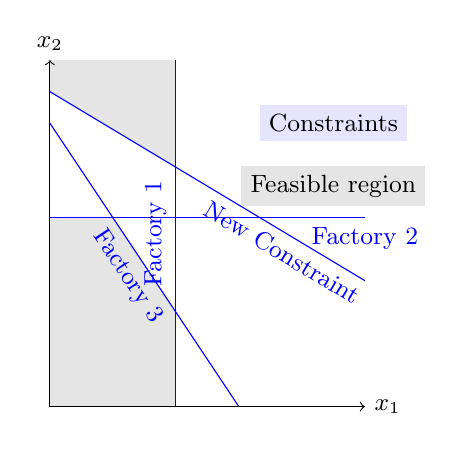
\begin{tikzpicture}[scale=0.4,every node/.style={font=\small}]
                        % Filling the feasible region
                        \fill[gray!20] (0,0) -- (0,6) -- (2,6) -- (4,3) -- (4,0) -- cycle;
                        \fill[gray!20] (0,11) -- (0,10) -- (4,7.6) -- (4,11) -- cycle;

                        % Constraints
                        \draw[blue] (4,0) -- (4,11) node[midway, left, sloped, above] {Factory 1};
                        \draw[blue] (0,12/2) -- (10,12/2) node[at end, below, sloped] {Factory 2};
                        \draw[blue] (0,9) -- (6,0) node[midway, below, sloped] {Factory 3};
                        % New Constraint: 3x1 + 5x2 >= 50
                        \draw[blue] (0,{50/5}) -- (10,{(50-3*10)/5}) node[midway,below right,sloped] {New Constraint};

                        % Axis
                        \draw[->] (0,0) -- (10,0) node[right] {$x_1$};
                        \draw[->] (0,0) -- (0,11) node[above] {$x_2$};

                        % Legends
                        \node at (9,9) [rectangle,fill=blue!10] {Constraints};
                        \node at (9,7) [rectangle,fill=gray!20] {Feasible region};
                    \end{tikzpicture}
                    \caption{The feasible region is defined by the area that satisfies \emph{all} constraints simultaneously.
                    Cannot be done, infeasible.}
                \end{figure}
            \end{column}
        \end{columns}

    \end{frame}


    \begin{frame}{Integer Programming and LP Relaxation}

        \begin{block}{LP Relaxation}
            \begin{itemize}
                \item A technique used to find an \emph{approximate} solution to an integer programming problem.
                \item Involves ignoring the integer constraint and solving the resulting linear program.
                \item The LP relaxation provides a bound on the value of the optimal solution of the integer program.
                If the solution to the LP relaxation happens to be integer, it is also a solution to the IP.
                \item The solution to the LP relaxation can be used as a starting point for other algorithms,
                like branch and bound, to find the integer solution.
            \end{itemize}
        \end{block}


    \end{frame}



    \begin{frame}{Binary Integer Programming (BIP)}
        \begin{block}{Binary Variables in BIP}
            Binary Integer Programming is a special case of Integer Programming where decision variables can take
            only values of 0 or 1.
            \begin{itemize}
                \item Represent binary decisions, e.g., do or do not.
                \item Often used to activate or deactivate constraints or other decision variables.
                \item Commonly denoted as \( y \) (referred to as \emph{auxiliary variables}), with main decision
                variables as \( x \).
            \end{itemize}
        \end{block}
        \framebreak
        \begin{block}{Example Usages}
            \begin{enumerate}
                \item \textbf{Either-Or Decisions:} If a company can open a factory or a retail store, but not both.
                \item \textbf{Fixed Costs:} If opening a factory incurs a fixed cost, \( y \) can indicate whether
                the factory is opened or not.
                \item \textbf{Set Values:} Selling products in predefined bundles (e.g. 6-packs).
            \end{enumerate}
        \end{block}
    \end{frame}
    \begin{frame}{Big M Method: Either-Or Constraints}
        \small

        Use the \emph{Big M} method with an auxiliary binary variable \( y \) to enforce one of two constraints:
        \begin{itemize}
            \item \( y = 1 \): Constraint A active, B non-binding.
            \item \( y = 0 \): Constraint B active, A non-binding.
        \end{itemize}

        Given:
        \begin{align*}
            Ax &\leq b & \text{(A)} \\
            Cx &\leq d & \text{(B)}
        \end{align*}

        Modify as:
        \begin{align*}
            Ax &\leq b + My \\
            Cx &\leq d + M(1-y)
        \end{align*}

        Choose \( M \) sufficiently large.


    \end{frame}

    \begin{frame}{Elevator Pitch: MIP in Daily Life}

        \begin{block}{Objective}
            Develop a 30-second pitch for a real-life mixed integer programming problem.
        \end{block}

        \begin{itemize}
            \item \textbf{Relatability}: Choose a daily life problem that most can resonate with.
            \item \textbf{Hook}: Begin with an engaging statement or question.
            \item \textbf{Problem Description}: Clearly state the problem.
            \item \textbf{Benefits}: Emphasize how solving it would improve daily life.
            \item \textbf{MIP Relevance}:
            \begin{itemize}
                \item Decision variables: Real, integer, binary.
                \item Linear constraints only.
            \end{itemize}
        \end{itemize}

        \begin{columns}
            \begin{column}{.5\textwidth}
                \begin{block}{Pointers}
                    \begin{itemize}
                        \item Engage the listener quickly.
                        \item Keep it concise and to the point.
                        \item Practice to ensure confidence and timing.
                    \end{itemize}
                \end{block}
                \footnotesize{Remember: This is about conveying the importance of the problem, not the solution details.}
            \end{column}
            \begin{column}{.5\textwidth}
                \begin{figure}
                    \centering
                    
\includegraphics[height=0.7\textheight]{figures/elevator-pitch.jpg}
                    %\caption{DALL-E: In a cartoon elevator, a snazzy cat with big glasses pitches to an executive
                    %kangaroo with a monocle. The cat, holding a doodled tablet about mixed integer programming,
                    %gestures excitedly. The kangaroo, leaning down with a hand on its chin, contemplates the cat's
                    %animated proposal.}
                \end{figure}
            \end{column}
        \end{columns}
    \end{frame}

\end{document}
